\documentclass[10pt,aspectratio=169]{beamer}
% Packages
\usepackage{mathabx}
\usepackage{xcolor}
\usepackage{amsmath}
\usepackage{mathtools}
\usepackage{standalone}
\usepackage{mhchem}
\usepackage{textpos}
\usepackage{graphicx}
\usepackage{wrapfig}
\usepackage{booktabs}
\usepackage{textcomp}
\usepackage{makecell}
\usepackage{wasysym}
\graphicspath{{images}}

% Configure template
\setbeamertemplate{navigation symbols}{}

% Theme
\usetheme[progressbar=frametitle]{metropolis}
\setbeamertemplate{caption}[numbered]
\setbeamersize{text margin left=5mm,text margin right=5mm}

% Title page details:
\title{Scientific Computing: Molecular dynamics}
\subtitle{Problemsheet 4}
\author{Jimin Kim, Christian Nix, Noah Schlenker}
\date{21. June 2024}
\institute{Technical University of Munich}

\begin{document}

% Title page frame
    \maketitle

    \addtobeamertemplate{frametitle}{}{
        \begin{textblock*}{100mm} (.945\textwidth,-.85cm)
            
\includegraphics[scale=0.14]{../template/res/tum_logo.png}
        \end{textblock*}}

% Outline frame
    \begin{frame}{Outline}
        \tableofcontents
    \end{frame}

% Slides
    
\section{Thermostat}
\label{sec:thermo}

\begin{frame}
    \frametitle{Thermostat}
    \begin{itemize}
        \item Adjusts particle velocities for temperature control
        \item Frequency control for temperature updates on simulation level
        \item Optimized by excluding divisions by 2 in $E_{kin}$
        \item $T_{current} = \frac{2 \cdot \left(\sum_{i=1}^{\#particles} \frac{m_i \langle v_i, v_i \rangle}{2}\right)}{\#dimensions\ \cdot\ \#particles}$
        \item $T_{current} = \frac{2 \cdot \frac{1}{2}\ \left(\sum_{i=1}^{\#particles} m_i \langle v_i, v_i \rangle\right)}{\#dimensions\ \cdot\ \#particles}$
        \item $T_{current} = \frac{\sum_{i=1}^{\#particles} m_i \langle v_i, v_i \rangle}{\#dimensions\ \cdot\ \#particles}$
    \end{itemize}
\end{frame}
    
\section{Rayleigh-Taylor instability}
\label{sec:rayleigh}

\begin{frame}
    \frametitle{Rayleigh-Taylor simulation}

    Boundary interface specifies \texttt{preUpdateBoundaryHandling} and \texttt{postUpdateBoundaryHandling} function

    \vspace{7pt}
    \begin{columns}
        \begin{column}{.5\textwidth}
            \centering{\textbf{preUpdateBoundaryHandling}}
            \begin{itemize}
                \item Executed before any forces are calculated
                \item[] \!\!\!\!\!\!\!\!\! \textcolor{orange}{$\Rightarrow$} Add all required halo particles
                \item Map from \texttt{CellIndex} to manipulations of the cell index and particle position $\rightarrow$ particle position + shift = halo particle position
                \item If multiple periodic boundaries affect a cell, only one will perform all shifts
            \end{itemize}
        \end{column}

        \begin{column}{.5\textwidth}
            \centering{\textbf{postUpdateBoundaryHandling}}
            \begin{itemize}
                \item Called after all updates to the particles
                \item All inserted halo particles will be removed
                \item Only after all bounds have been applied the particle is within the domain (known end)
                \item[] \!\!\!\!\!\!\!\!\! \textcolor{orange}{$\Rightarrow$} Only then do update
            \end{itemize}
        \end{column}
    \end{columns}
    \vspace{7pt}

    \begin{itemize}
        \item New force calculation including gravitational force
        \item Simulation class \texttt{MixedLJSimulation} for multiple particle types:
        \begin{itemize}
            \item Uses Lorentz-Berthelot mixing rule for parameters during setup
            \item Includes thermostat for temperature update and initialization
        \end{itemize}
    \end{itemize}
\end{frame}

\begin{frame}
    \frametitle{Simulation observations}
    \begin{itemize}
        \item Noticeable Bouncing/Splashing when layers collide
        \item Top liquid forms drops initially while mixing
    \end{itemize}
    \begin{figure}
        \label{fig:bounce}
        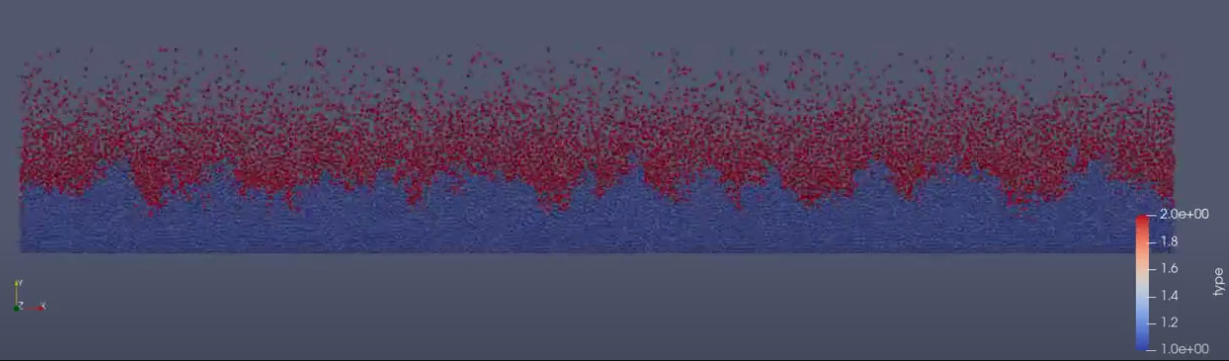
\includegraphics[width=0.9\textwidth]{../../res/rayleigh_bounce}
    \end{figure}
\end{frame}
    
\section{Falling Drop - Liquid}
\label{sec:falling}

\begin{frame}
    \frametitle{Falling Drop - Liquid}
    \begin{itemize}
        \item Checkpointing by saving simulation state in XML format via \texttt{XmlWriter}
        \item First with thermostat: Slow descent and calm assimilation, interesting wave patterns!
        \item Without temperature regulation: Rapid fall and violent splash, significant wave reflection from boundaries!
        \item With periodic boundaries: Negligible differences, waves splash against each other like reflection boundary
    \end{itemize}
\end{frame}
    
\section{Performance test}
\label{sec:perf}

\begin{frame}
    \frametitle{Google Benchmark}
    \begin{table}
        \centering
    \begin{tabular}{|c|c|c|c|}
        \toprule
        Benchmark/\#Particles & Time & CPU & Iterations \\
        \toprule
        BM\_LJSimulation/1000 & 1.4485e+10 ns & 1.4477e+10 ns & 1 \\
        \midrule
        BM\_LJSimulation/2000 & 5.7983e+10 ns & 5.7959e+10 ns & 1 \\
        \midrule
        BM\_LJSimulation/4000 & 2.3180e+11 ns & 2.3171e+11 ns & 1 \\
        \midrule
        BM\_LJSimulation/8000 & 9.2722e+11 ns & 9.2686e+11 ns & 1 \\
        \midrule
        BM\_LJSimulation\_BigO & 14487.81 $N^2$ & 14482.20 $N^2$ & - \\
        \midrule
        BM\_LinkedLJSimulation/1000 & 28515871 ns & 28493193 ns & 25 \\
        \midrule
        BM\_LinkedLJSimulation/2000 & 54951418 ns & 54934137 ns & 13 \\
        \midrule
        BM\_LinkedLJSimulation/4000 & 114455900 ns & 114424760 ns & 6 \\
        \midrule
        BM\_LinkedLJSimulation/8000 & 236827726 ns & 236733811 ns & 3 \\
        \midrule
        BM\_LinkedLJSimulation\_BigO & 29304.28 $N$ & 29293.31 $N$ & - \\
        \bottomrule
    \end{tabular}
    \end{table}
\end{frame}

\begin{frame}
    \frametitle{Graphs}
    \textbf{Results show improvement from squared to linear runtime!}
    \begin{figure}
        \label{fig:timelc}
        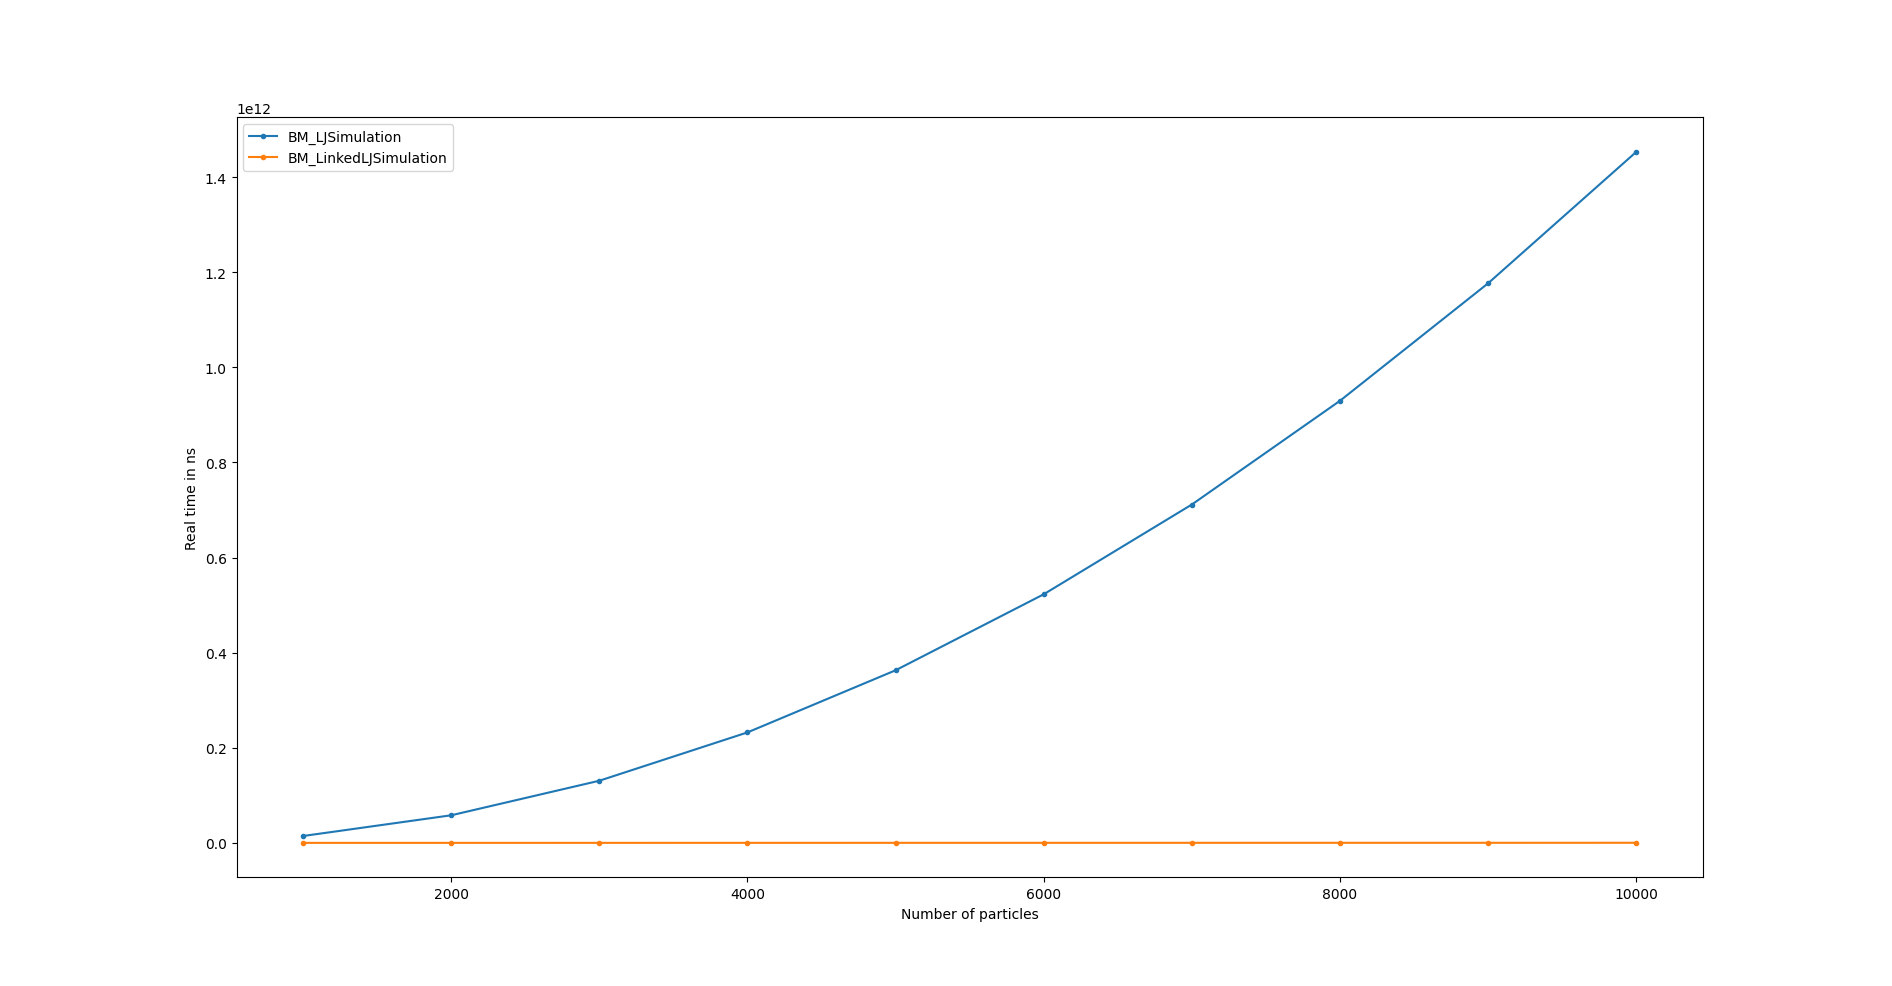
\includegraphics[width=0.9\textwidth]{res/lj_big_plot_linear}
    \end{figure}
\end{frame}

\begin{frame}
    \frametitle{Graphs}
    \begin{figure}
        \label{fig:timelclog}
        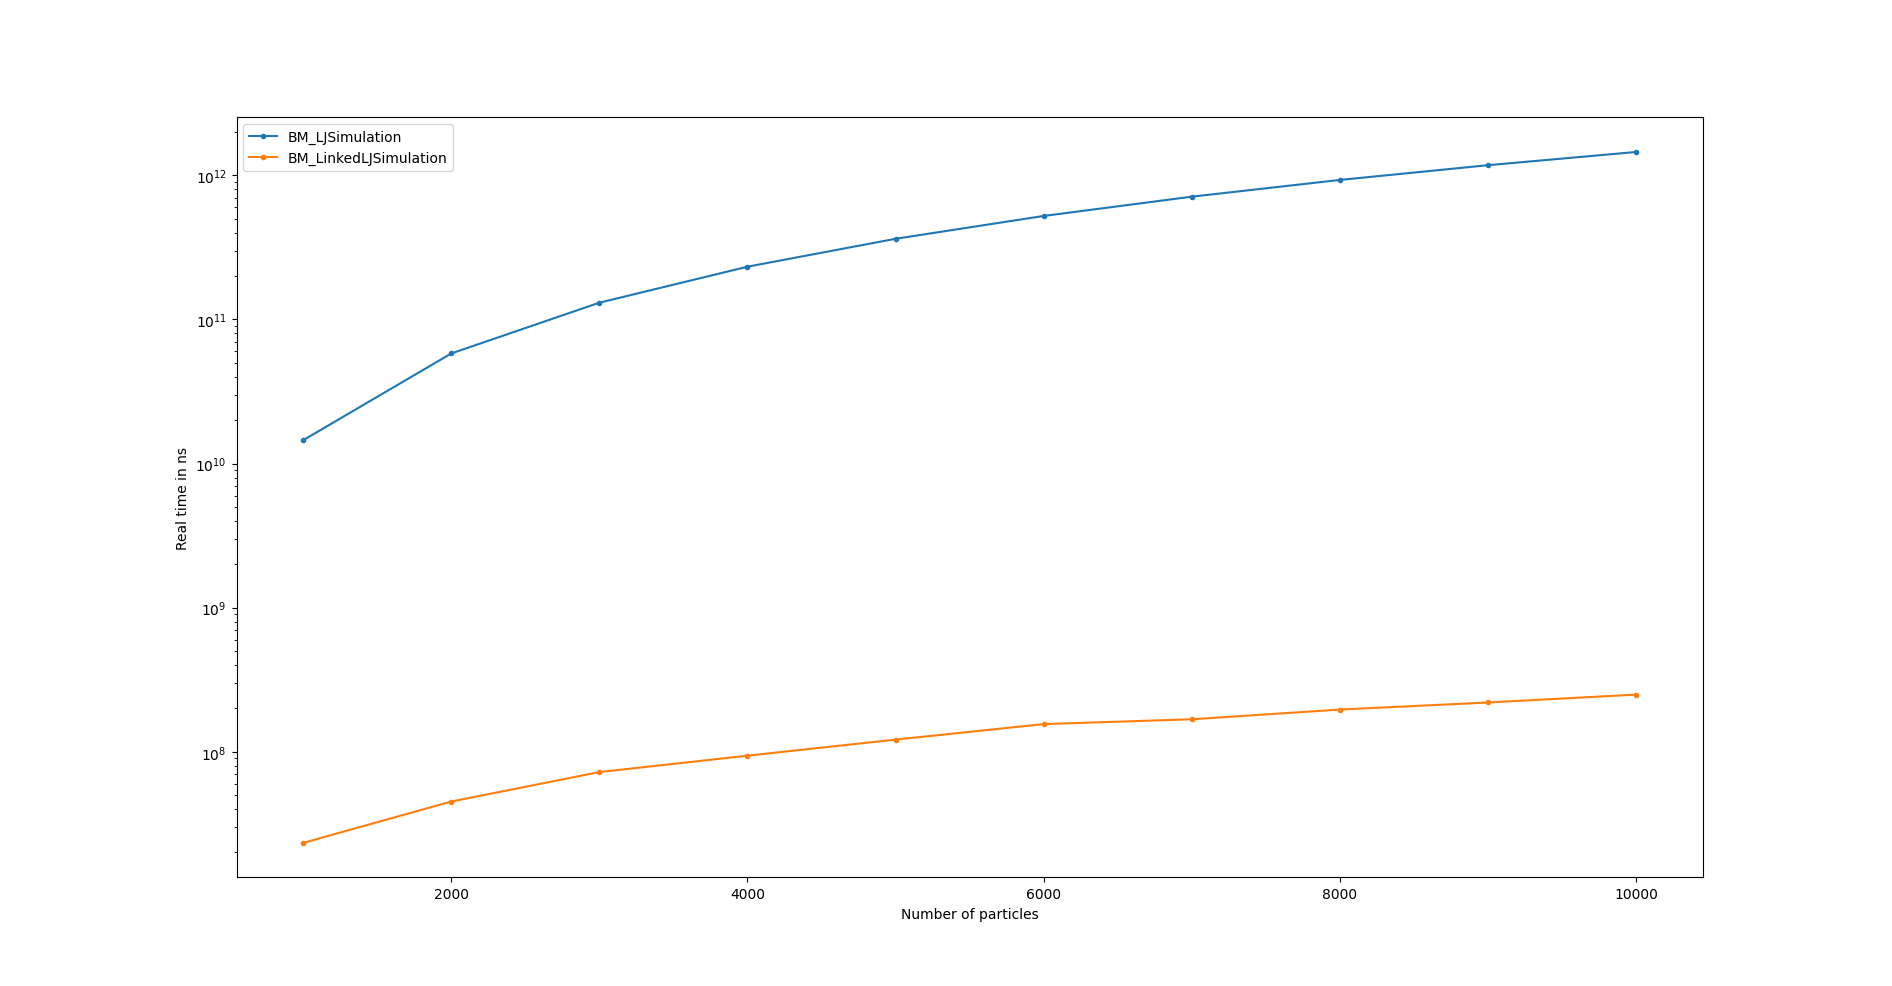
\includegraphics[width=0.9\textwidth]{res/lj_big_plot_log}
    \end{figure}
\end{frame}

    
\section{Optimization}
\label{sec:opt}

\begin{frame}
    \frametitle{Optimizations}
    \begin{itemize}
        \item Optimizations through inlining: Costs of function calls reduced
        \item More efficient check for cutoff radius by saving root calculations and using squared cutoff radius.
    \end{itemize}
\end{frame}

\end{document}